Te topic of motion planing is a widely researched topic, with multiple algorithm formulated to compute the optimal motion for a vehicle A, to go from points B to C. But first we must note the difference between path planing and trajectory planing, a path is simply a collection of points describing how to move from one place to another, without any information related to time. A trajectory provides notion on time of the trajectory, and must be able to take into consideration the dynamics of a vehicle\cite{wolek2017model}.

In\cite{lavalle2006planning} a way of mathematicaly formalazing a motion plan in present. For the case of this work, we would define the space of all configuration $\mathcal{C}$, in this space we have an agent $\mathcal{R}$  moving in an environment $\mathcal{W} = \mathbb{R}^3$ and a set of obstacles $\mathcal{O} = \begin{Bmatrix} \mathcal{O}^{1} \dots \mathcal{O}^{N}\end{Bmatrix}$, it is important to note that the obstacle are both static and moving. We can represent the configuration of the agent as $H = (x_{t}, y_{t}, z_{t}, q)$,  where q represent the orientation of the agent, in quaterion form 

The obstacle region, $\mathcal{C}_{obs} \subseteq \mathcal{C}$ is defined as, $\mathcal{C}_{obs} = \left\{  h \in \mathcal{C} \vert A(h) \cap \mathcal{O} \ne \emptyset \right\}$, and this is the list of all possible configuration of the agent that would result in a intersection with a the obstacle regions. The left over configuration can be defined as free space, meaning $\mathcal{C}_{free} = \mathcal{C} \setminus \mathcal{C}_{obs}$.

This situation is much more complex when our robot is composed by more than on body, since we not only want to avoid colisions between the robots and the obstacles, but also in between the multiple bodies. We must model our robot not only as a single agent $\mathcal{A}$, but rather a set of agents, $\left\{ \mathcal{A}_1 \dots \mathcal{A}_m \right\}$, wit this we can now denote the set of the colition pair, (i, i) $\in \mathcal{P}$, where $ i, j \in {1, \dots, m}, \text{ with } i \ne j$. The set $\mathcal{P}$ can not represent all the pair, since link that are rigidly connected will always be in contact with one another, this means we not have our obstacle space being defined as in \ref{eq:background:trajectory generation:obstacle space}. With the definition of the space we now only need to be able to compute a trajectory moving in between the objective configuration and the initial configuration $\in \mathcal{C}_{free}$.

\begin{equation}
    \mathcal{C}_{obs} = \left( \overset{m}{\underset{i=1}{\cup}}\{h \in \mathcal{C} \vert \mathcal{A}_i(h) \cap \mathcal{O} \neq \emptyset \} \right) \cup \left( \underset{[i, j] \in \mathcal{P}}{\cup} \{ h \in \mathcal{C} \vert \mathcal{A}_i(h) \cap \mathcal{A}_j(h) \neq \emptyset\}  \right)
    \label{eq:background:trajectory generation:obstacle space}
\end{equation}



\subsubsection{Motion Planing algorithms}

The scheme we can see in figure \ref{fig:background:trajectory generation:motion planning algorithms}, is a copy of a scheme in \cite{InesBatista2022Thesis}, in this a work a collection of multiple motion planning algorithm is compiled explain their working and their main advantages and disadvantages. For this work we will focus only a few of the search based methods, in this specific case Djikstra, $A^{*}$ and $D^{*}$, and then from the sampling based group we will focus on RRT and variations and PRM.

\paragraph{Search based methods}

Search based algorithm\cite{latombe2012robot}, divide $\mathcal{C}_{free}$ into a finite number of cells. We then create a connectivity graph, G = (V, E), that is capable of representing adjacency between the cells. This means, the finite number of cell we have are represented by all the vertices, set V, and the edges, set E, represent the connection between two different cells. We can then run any type of graph search algorithm, a good examples of it are the aformentioned $D^{*}$, $A^{*}$ \cite{A-start-original} and Djjiikstra\cite{dijkstra2022note}.

\textbf{Djikstra} is a complete algorithm, meaning if one single solution exists, it will find it, that has the objective of finding the shortest path between two points in graph, the main problem we have in this algorithm is the computational cost grows quadratically with the increase of the search space. \textbf{$A^{*}$} is a variation of Djikstra, that uses a heuristic to guide the search, this means that the computational cost is reduced, but the algorithm is not complete, meaning it may not find a solution if one exists. \textbf{$D^{*}$} is a variation of $A^{*}$, that is capable of reusing the information from previous searches, this means that if replanning is needed, the second search will be much faster since we can reuse information previously computed. With those algorithms we can guarantee optimality, but only when working in a discrete space, and with a high computational cost. 

\paragraph{Sampling based methods} are a good approach when working with planning motion problems for robots. 



\paragraph{Sampling based methods}

\begin{figure}[H]
    \centering
    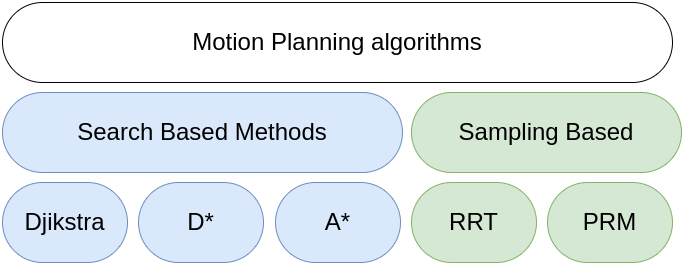
\includegraphics[width=0.7\textwidth]{Images/Background/Trajectory Generation/Motion_planing_algorithms.drawio.png}
    \caption{Scheme of motion planning algorithm}
    \label{fig:background:trajectory generation:motion planning algorithms}
\end{figure}

